%!TEX root = ../../../memoria.tex
\subsection{\dashboardEF}
Corresponde al administrador de características de la aplicación. Básicamente muestra toda las funcionalidades customizables que existen en la plataforma.
Cada package agregado el proyecto contiene el archivo \packageDescriptionFILE el cuál proporciona al \dashboardEF la información necesaria para agregar una o más componentes a la \uiSiglaAS con información descriptiva y con el link hacía la pantalla de configuración.
La información que se muestra de cada componente corresponde a:

\begin{itemize}
	\item Nombre de la componente a agregar.
	\item Descripción breve de la componente.
	\item Un icono 
\end{itemize} 


\begin{figure}[H]
	\centering
	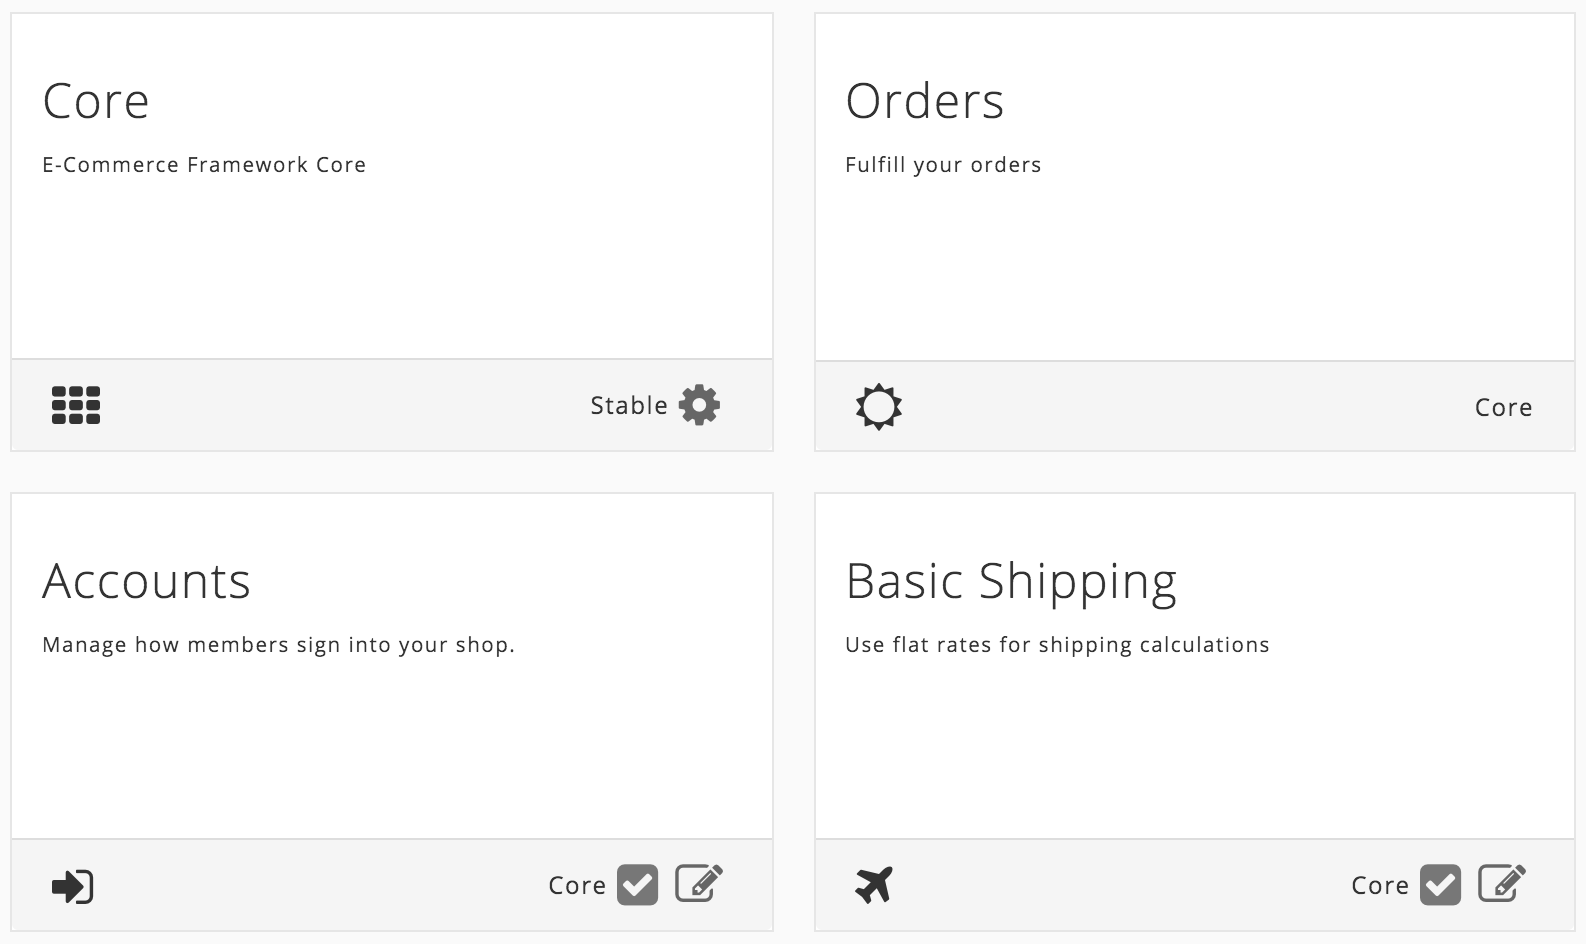
\includegraphics[width=0.8\textwidth]{figuras/dashboard/dashboard_menu.png}
	\caption{\dashboardEF con elementos configurables de la aplicación.}
	\label{figure:dashboard:dashboard_menu}
\end{figure}

En la \refFigura{figure:dashboard:dashboard_menu} se observan 4 elementos configurables de la aplicación. 

\subsubsection{\ecomFrameworkCoreEF}

Corresponde a la customización de los elementos relacionados directamente con la tienda. La información se ha jerarquizado en diferentes paneles de contenido plegable (conocidos como menú acordeón) los cuales se observan en la \refFigura{figure:dashboard:ecommerce:main_menu}.
%Displays collapsible content panels for presenting information in a limited amount of space.
\begin{figure}[H]
	\centering
	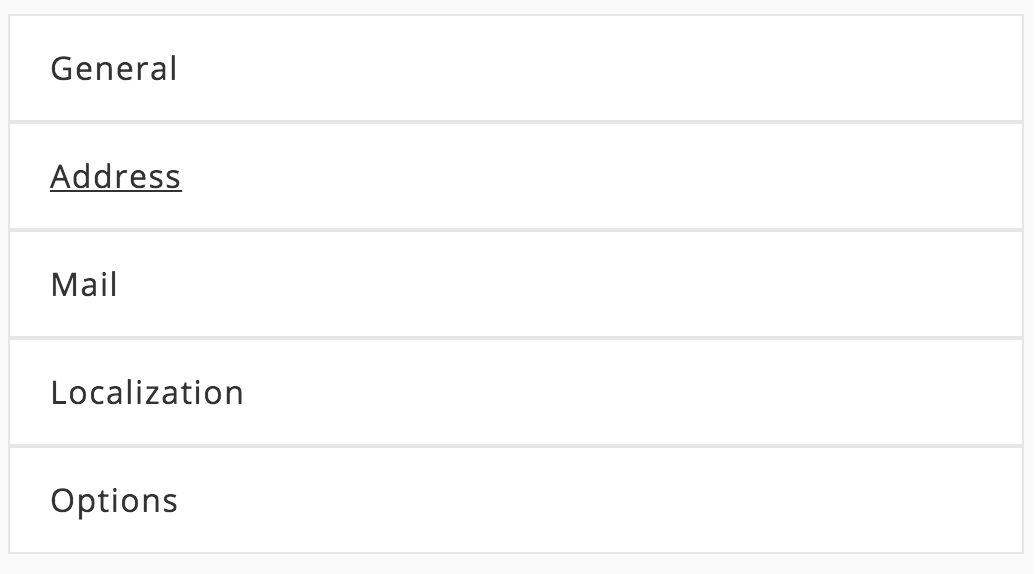
\includegraphics[width=0.6\textwidth]{figuras/dashboard/ecommerce/main_menu.png}
	\caption{Menú general de \ecomFrameworkCoreEF.}
	\label{figure:dashboard:ecommerce:main_menu}
\end{figure}

Cada uno de estos elementos tiene información configurable, además del \feedback habitual correspondiente a la información entregada de validación de cada campo, tiene una ventana emergente para indicar si la actualización del formulario fue o no exitosa.
La rázon de esta información extra es muy sencilla, si no existieran estos mensajes emergentes, estaría la ambigüedad de si el resultado fue exitoso o no dado que no hay ningún otro elemento gráfico con el cual se podría inferir el resultado. Por ejemplo, el formulario no se \'limpia\', el formulario no se cierra, no se agrega un nuevo elemento a una lista, etc.

\begin{figure}[H]
	\centering
	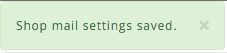
\includegraphics[width=0.6\textwidth]{figuras/dashboard/ecommerce/success_message.png}
	\caption{Mensaje de confirmación de éxito en la actualización del formulario. Este mensaje se esconde después de un breve intervalo de tiempo.}
	\label{figure:dashboard:ecommerce:success_message}
\end{figure}

\begin{figure}[H]
	\centering
	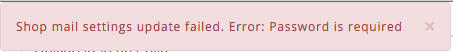
\includegraphics[width=0.8\textwidth]{figuras/dashboard/ecommerce/error_message.png}
	\caption{Mensaje para informar sobre un error en el proceso de actualización del formulario.}
	\label{figure:dashboard:ecommerce:error_message}
\end{figure}

En el caso de ser exitoso, aparece un mensaje el cual eventualmente desaparecerá de un breve intervalo de tiempo(\refFigura{figure:dashboard:ecommerce:success_message}). Los mensajes de error persisten en el tiempo. Por lo tanto se deben cerrar para que desaparezcan (\refFigura{figure:dashboard:ecommerce:error_message}).


\subsubsection*{Panel \generalPanel}

El panel general está formado por dos formularios; el primero solo contiene un campo y es un checkbox para permitir que un usuario \userGuestAccount pueda realizar un \checkoutCOM (\refFigura{figure:dashboard:ecommerce:general_menu:allow_checkout}).

\begin{figure}[H]
	\centering
	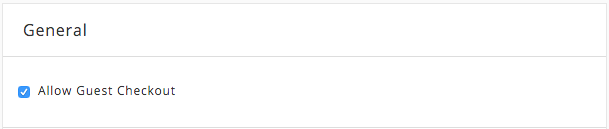
\includegraphics[width=0.6\textwidth]{figuras/dashboard/ecommerce/general_menu/allow_checkout.png}
	\caption{Formulario de información general de la tienda}
	\label{figure:dashboard:ecommerce:general_menu:allow_checkout}
\end{figure}

Este formulario tiene la particuladidad que se envía automáticamente al cambiar su estado.
El otro formulario está relacionado con la información más general de la empresa ( \refFigura{figure:dashboard:ecommerce:general_menu:menu})

\begin{figure}[H]
	\centering
	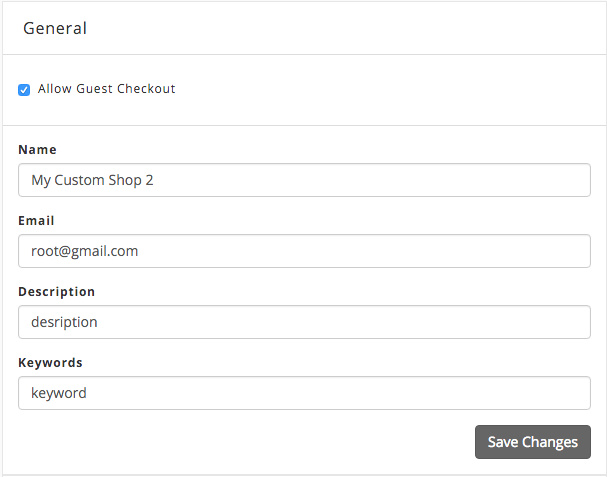
\includegraphics[width=0.6\textwidth]{figuras/dashboard/ecommerce/general_menu/menu.png}
	\caption{Formulario de información general de la tienda}
	\label{figure:dashboard:ecommerce:general_menu:menu}
\end{figure}

\begin{table}[H]
    \centering
	\begin{tabular}{ |l|c||l| }
		\hline Campo & Requerido & Restricción \\ \hline
		\multirow{1}{*}{\textit{Name}} 			&  {\checkmark} &  \\ \hline
		\multirow{1}{*}{\textit{Email}} 		&  				&  Debe ser un email válido.\\ \hline
		\multirow{1}{*}{\textit{Description}} 	&  				&  \\ \hline
		\multirow{1}{*}{\textit{Keywords}} 		&  				&  \\ \hline
		\hline
	\end{tabular}
 	\caption{Restrincciones formulario \generalPanel}
    \label{tab:dashboard:ecommerce:form:general}
\end{table}


Este formulario solo tienen un campo obligatorio, y corresponde a \textit{Name}. Al igual que otros formularios, dicho campo se destaca de color rojo, además de entregar un mensaje a modo de identificar el error (\refFigura{figure:apendice:dashboard:ecommerce:general_menu:updated_error}).



\subsubsection*{Panel \addressPanel}\label{capitulo:solucionImplementada:dashboard:subsubsection:addressPanel}

Este formulario se utiliza para agragar información física de la tienda, como algún teléfono de contacto.

\begin{figure}[H]
	\centering
	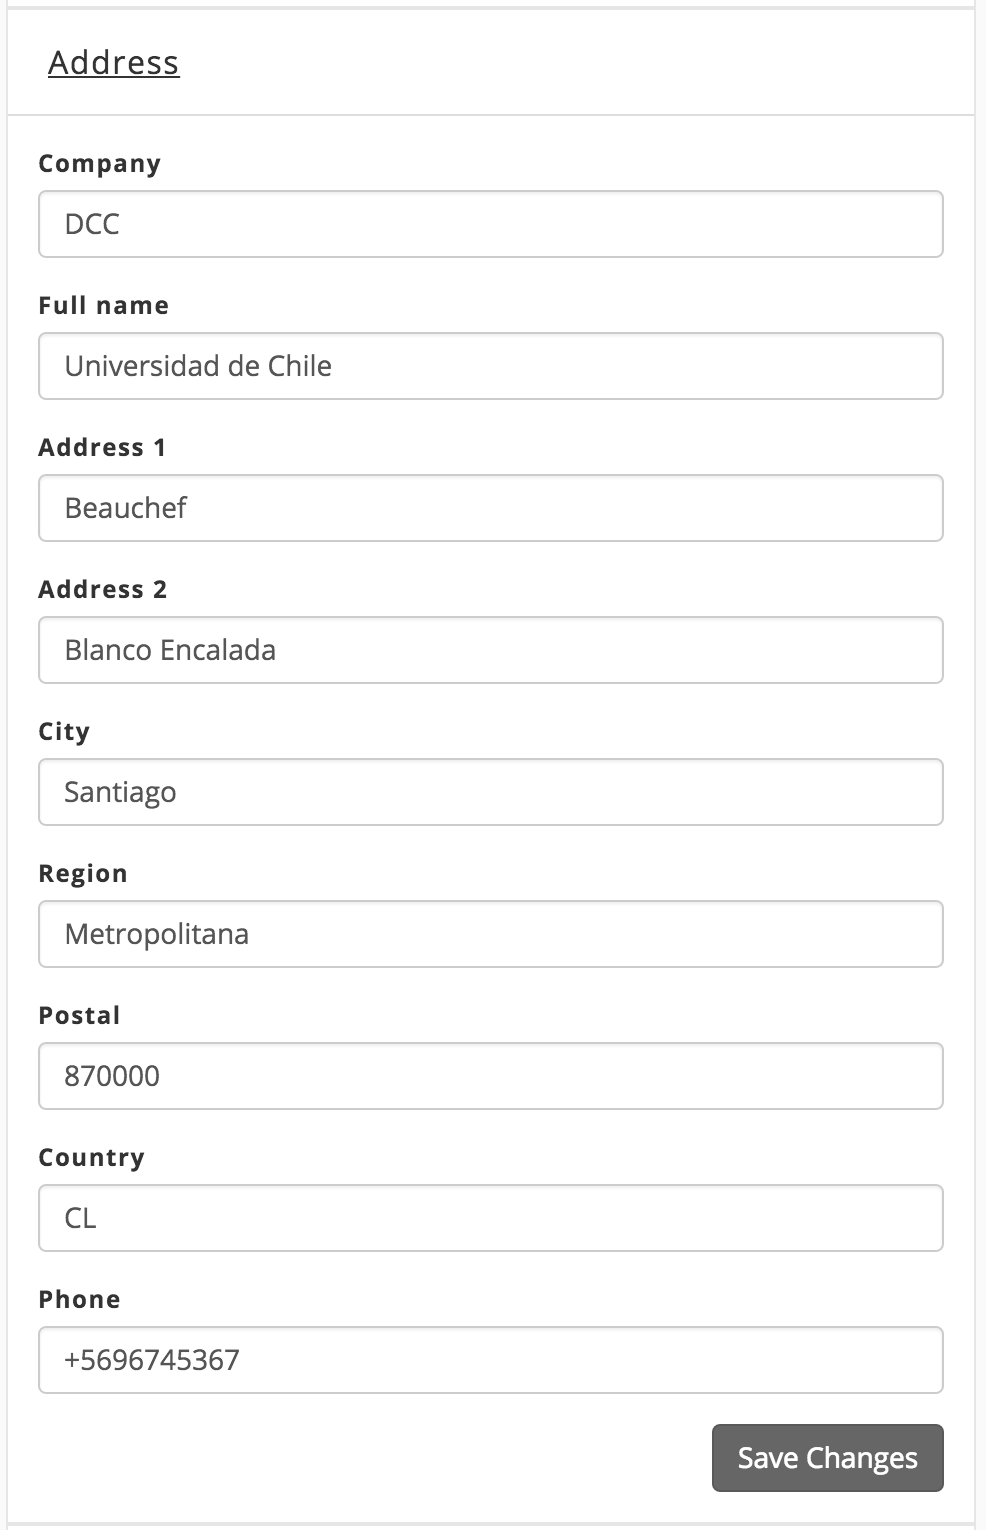
\includegraphics[width=0.5\textwidth]{figuras/dashboard/ecommerce/address/menu.png}
	\caption{Formulario de la dirección física de la tienda.}
	\label{figure:dashboard:ecommerce:address:menu}
\end{figure}

En relación a los campos del formulario, se tienen las siguientes restricciones (\reftabla{tab:dashboard:ecommerce:form:address}):

\begin{table}[H]
    \centering
	\begin{tabular}{ |l|c||l| }
		\hline Campo & Requerido & Restricción \\ \hline
		\multirow{1}{*}{\textit{Full name}} &  {\checkmark} &  \\ \hline
		\multirow{1}{*}{\textit{Address 1}} &  {\checkmark} &  \\ \hline
		\multirow{1}{*}{\textit{Address 2}} &   			&  \\ \hline
		\multirow{1}{*}{\textit{City}} 		&  {\checkmark} &  \\ \hline
		\multirow{1}{*}{\textit{Region}} 	&  {\checkmark} &  \\ \hline
		\multirow{1}{*}{\textit{Postal}} 	&  {\checkmark} &  \\ \hline
		\multirow{1}{*}{\textit{Country}}	&  {\checkmark} &  \\ \hline
		\multirow{1}{*}{\textit{Phone}} 	&  {\checkmark} &  \\ \hline
	\end{tabular}
 	\caption{Restrincciones formulario \addressPanel}
    \label{tab:dashboard:ecommerce:form:address}
\end{table}


\subsubsection*{Panel \mailPanel}

Corresponde a la información básica necesaria para configurar un servicio de \email. Agregar un \email no es requerido, pero si se configura el servicio deben agregarse tódos los campos(\reftabla{tab:dashboard:ecommerce:form:mail}).

\begin{figure}[H]
	\centering
	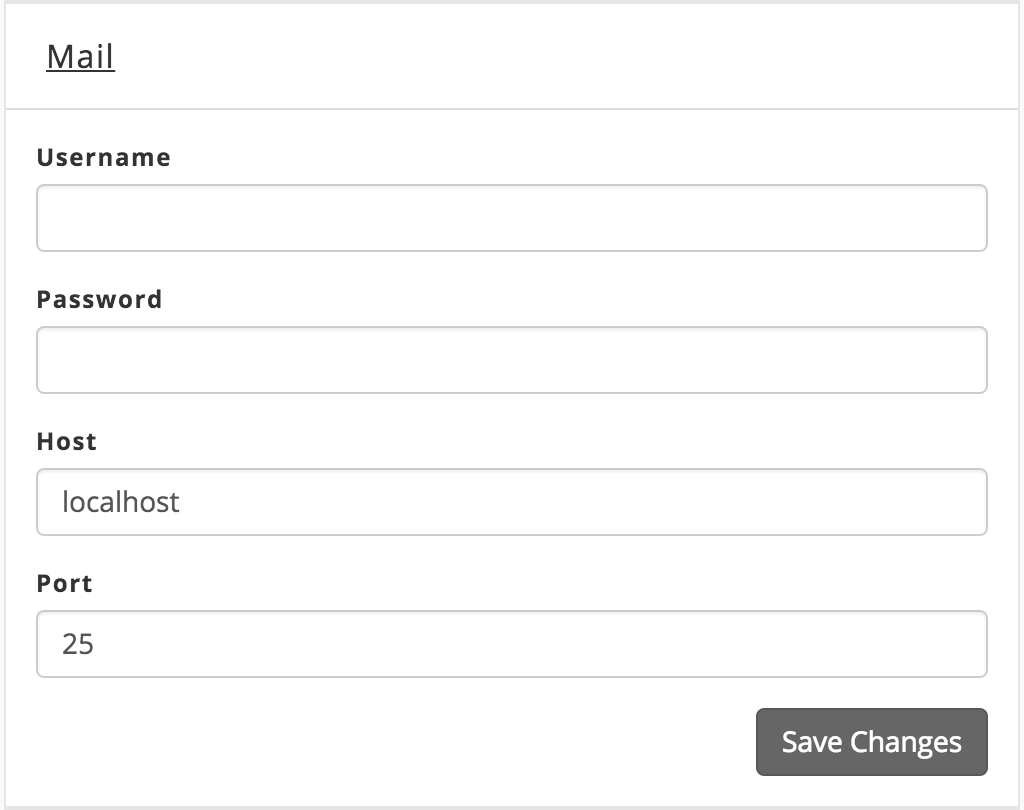
\includegraphics[width=0.6\textwidth]{figuras/dashboard/ecommerce/mail/menu.png}
	\caption{Formulario con la información de la configuración del Mail.}
	\label{figure:dashboard:ecommerce:mail:menu}
\end{figure}

\begin{table}[H]
    \centering
	\begin{tabular}{ |l|c||l| }
		\hline Campo & Requerido & Restricción \\ \hline
		\multirow{1}{*}{\textit{User Name}} &  {\checkmark} &  \\ \hline
		\multirow{1}{*}{\textit{Password}} 	&  {\checkmark} &  \\ \hline
		\multirow{1}{*}{\textit{Host}} 		&  {\checkmark} &  \\ \hline
		\multirow{1}{*}{\textit{Port}} 		&  {\checkmark} & Número mayor que 0 \\ \hline
		\hline
	\end{tabular}
 	\caption{Restrincciones formulario \mailPanel}
    \label{tab:dashboard:ecommerce:form:mail}
\end{table}


\subsubsection*{Panel \optionsPanel}

\begin{figure}[H]
	\centering
	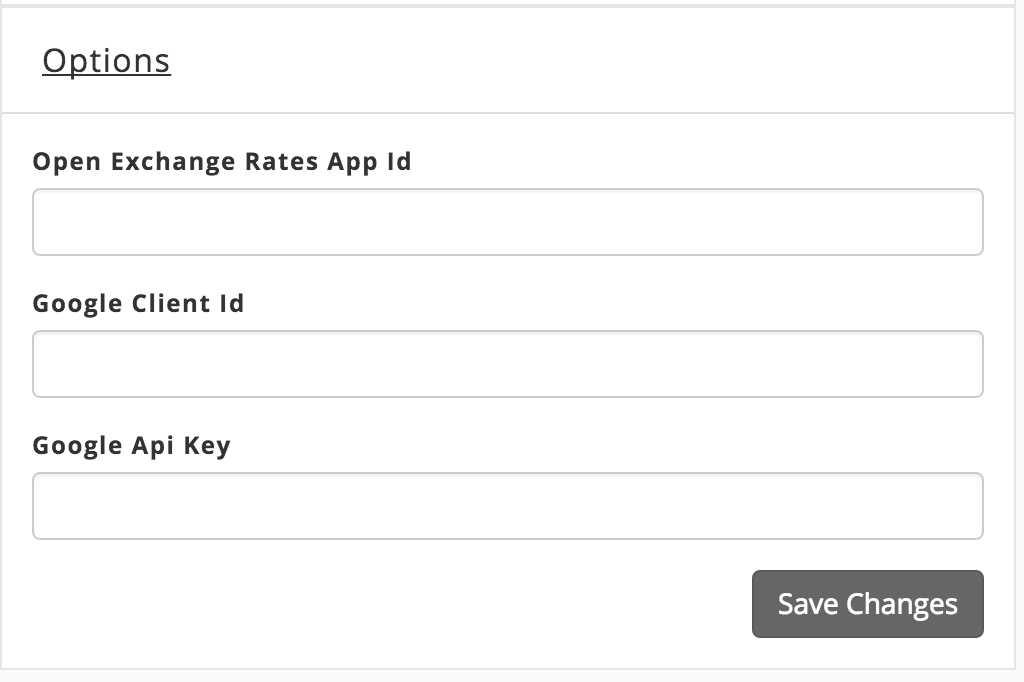
\includegraphics[width=0.6\textwidth]{figuras/dashboard/ecommerce/options/menu.png}
	\caption{Formulario con información relacionada con los Analytics.}
	\label{figure:dashboard:ecommerce:options:menu}
\end{figure}

\begin{table}[H]
    \centering
	\begin{tabular}{ |l|c||l| }
		\hline Campo & Requerido & Restricción \\ \hline
		\multirow{1}{*}{\textit{Open Exchange}} 	&  {\checkmark} &  \\ \hline
		\multirow{1}{*}{\textit{Google Client}} 	&  {\checkmark} &  \\ \hline
		\multirow{1}{*}{\textit{Google Api}} 		&  {\checkmark} &  \\ \hline
		\hline
	\end{tabular}
 	\caption{Restrincciones formulario \optionsPanel}
    \label{tab:dashboard:ecommerce:form:options}
\end{table}

\subsection{\ordersEF}

	Por definición, una orden corresponde a una solicitud confirmada, en esta caso particular, desde un cliente para comprar un \itemCOM o servicio bajo unos términos y condiciones específicas. Es importante mencionar que el flujo de compra no ha terminado cuando el cliente a realizado el pago. Es en este escenario en donde surge el concepto de \orderFulfillmentCOM.
	Esta sección permite al encargado administrar las ordenes generadas por los clientes para posteriormente gestionarlas, conteniendo por lo tanto, toda la información necesaria para llevar a cabo dicho proceso.
	Dada la complejidad de operaciones que puede alcanzar \orderFulfillmentCOM, en la aplicación, está sección se ha simplificado a lo más fundamental.

	Al selección las Ordenes desde el panel de \dashboardEF, lo primero que se vera es la lista de todas las Ordenes ingresadas por los clientes que se encuentran actualmente en el sistema. En la \refFigura{figure:dashboard:orders:grid} se ve la pantalla de Ordenes.


	\begin{figure}[H]
		\centering
		\includegraphics[width=0.6\textwidth]{figuras/dashboard/orders/grid.png}
		\caption{Vista general de todas las ordenes ingresadas por clientes.}
		\label{figure:dashboard:orders:grid}
	\end{figure}

	Cada una de estas ordenes estan disponibles para realiar acciones sobre ellas. Estas acciones radican principalmete en cambiar el estado actual de la orden. El detalle de la orden se ve en la \refFigura{figure:dashboard:orders:orderInfo}
%TODO agregar mas información sobre la orden.
	\begin{figure}[H]
		\centering
		\includegraphics[width=0.6\textwidth]{figuras/dashboard/orders/orderInfo.png}
		\caption{Detalle de orden ingresada por un cliente.}
		\label{figure:dashboard:orders:orderInfo}
	\end{figure}


\subsection{\accountsEF}

	Permite agregar o quitar permisos a los usuarios. El sistema actualmente permite crear usuarios y modificar sus permisos permitiendo o eliminando las componentes relacionadas a sus permisos.

	\begin{figure}[H]
		\centering
		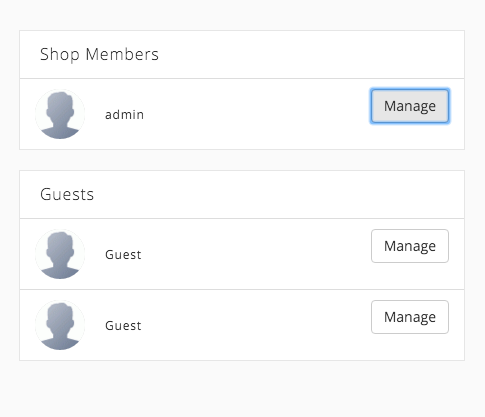
\includegraphics[width=0.6\textwidth]{figuras/dashboard/account/users.png}
		\caption{Interfaz con los usuarios del sistema.}
		\label{figure:dashboard:account:users}
	\end{figure}


	\begin{figure}[H]
		\centering
		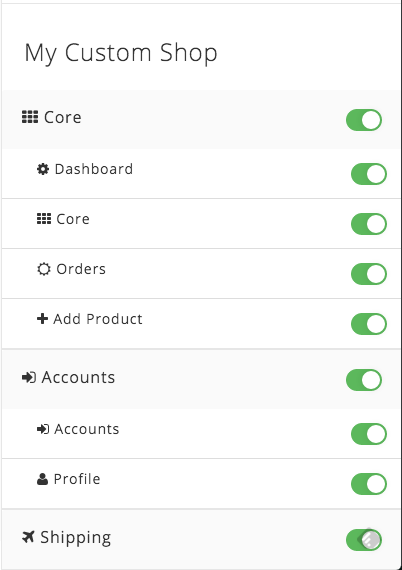
\includegraphics[width=0.6\textwidth]{figuras/dashboard/account/permisos.png}
		\caption{Interfaz para administrar los permisos del sistema.}
		\label{figure:dashboard:account:permisos}
	\end{figure}

\begin{table}[H]
    \centering
	\begin{tabular}{ |l|c||l| }
		\hline Campo & Requerido & Restricción \\ \hline
		\multirow{1}{*}{\textit{Core}} 			&  \checkmark 	& Boolean \\ \hline
		\multirow{1}{*}{\textit{Dashboard}} 	&  \checkmark	& Boolean \\ \hline
		\multirow{1}{*}{\textit{Orders}} 		&  \checkmark	& Boolean \\ \hline
		\multirow{1}{*}{\textit{Add Product}} 	&  \checkmark	& Boolean \\ \hline
		\multirow{1}{*}{\textit{Accounts}} 		&  \checkmark	& Boolean \\ \hline
		\multirow{1}{*}{\textit{Profile}} 		&  \checkmark	& Boolean \\ \hline
		\multirow{1}{*}{\textit{Shipping}} 		&  \checkmark	& Boolean \\ \hline
	\end{tabular}
 	\caption{Resumen restrincciones formulario para los permisos.}
    \label{tab:dashboard:account:form:restrictions:account}
\end{table}


\subsection{\shippingEF}\label{cap:solucionImplementada:section:}

\shippingEF es parte del proceso realmente grande y complejo perteneciente al \workflowCPT \orderFulfillmentCOM. 

Como primer paso, hay que agregar una dirección de origen, la cual es agreagada en \nameref{capitulo:solucionImplementada:dashboard:subsubsection:addressPanel}.

Segundo, se deben agregar \shippingZonesCOM los cuales tendran su correspondiente \shippingRatesCOM. Existen servicios que permiten calcular en tiempo real el \shippingRatesCOM, evitando así que la tienda asuma un costo extra por un error en la estimación de la tarifa de envío. El sitio además debería ser capaz de determinar, si la dirección de destino se encuentra dentro de alguna de las \shippingZonesCOM definidas.

% TODO falta agregar descripcion del proceso
%https://docs.shopify.com/manual/shipping/initial-shipping-setup#add-a-shipping-zone

Por temás de tiempo, se decidío simplificar la solución, permitiendo agregar diferentes opciones de \shippingEF que eventualmente representarían diferentes criterios de envío.

%TODO Agregar mas informaciñon 

\begin{figure}[H]
	\centering
	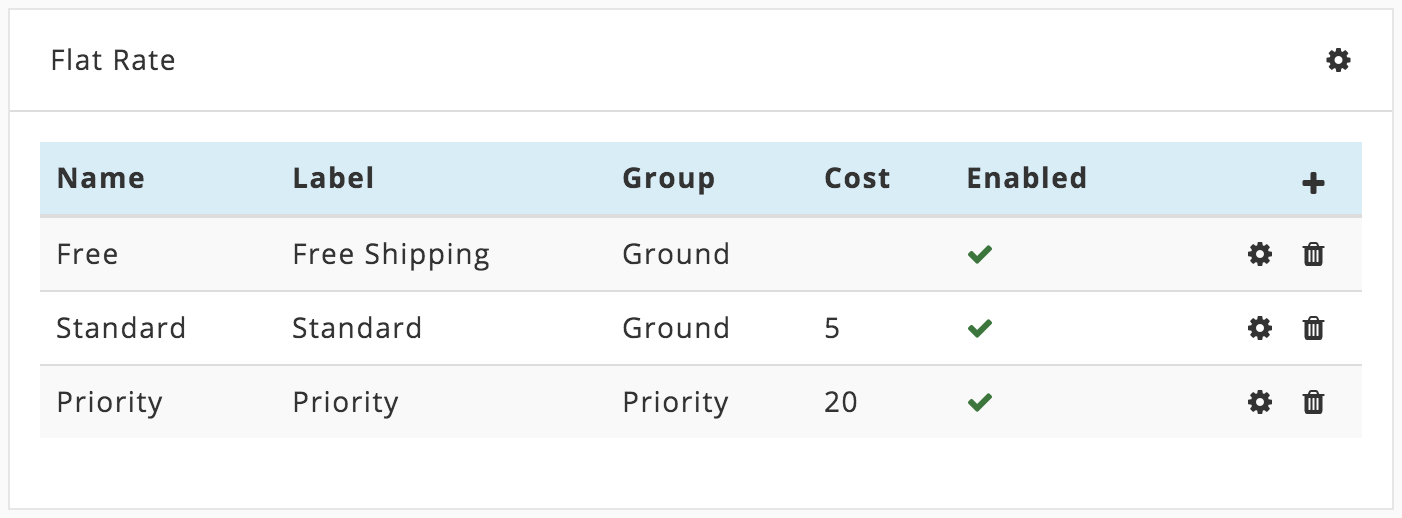
\includegraphics[width=0.6\textwidth]{figuras/dashboard/shipping/shipping_options.png}
	\caption{Tabla con todas las opciones de \shippingEF disponibles.}
	\label{figure:dashboard:shipping:shipping_options}
\end{figure}

\begin{table}[H]
    \centering
	\begin{tabular}{ |l|c||l| }
		\hline Campo & Requerido & Restricción \\ \hline
		\multirow{1}{*}{\textit{Method Name}} 	&  \checkmark 	& \\ \hline
		\multirow{1}{*}{\textit{Public Label}} 	&  \checkmark	& \\ \hline
		\multirow{1}{*}{\textit{Group}} 		&  \checkmark	& \\ \hline
		\multirow{1}{*}{\textit{Cost}} 			&  				& \\ \hline
		\multirow{1}{*}{\textit{Handling}} 		&  				& \\ \hline
		\multirow{1}{*}{\textit{Rate}} 			&  \checkmark	& Número mayor que 0. \\ \hline
		\multirow{1}{*}{\textit{Enabled}} 		&  \checkmark	& Boolean \\ \hline
	\end{tabular}
 	\caption{Resumen restrincciones formulario para \shippingEF.}
    \label{tab:dashboard:shipping:form:restrictions:shipping}
\end{table}

\begin{figure}[H]
	\centering
	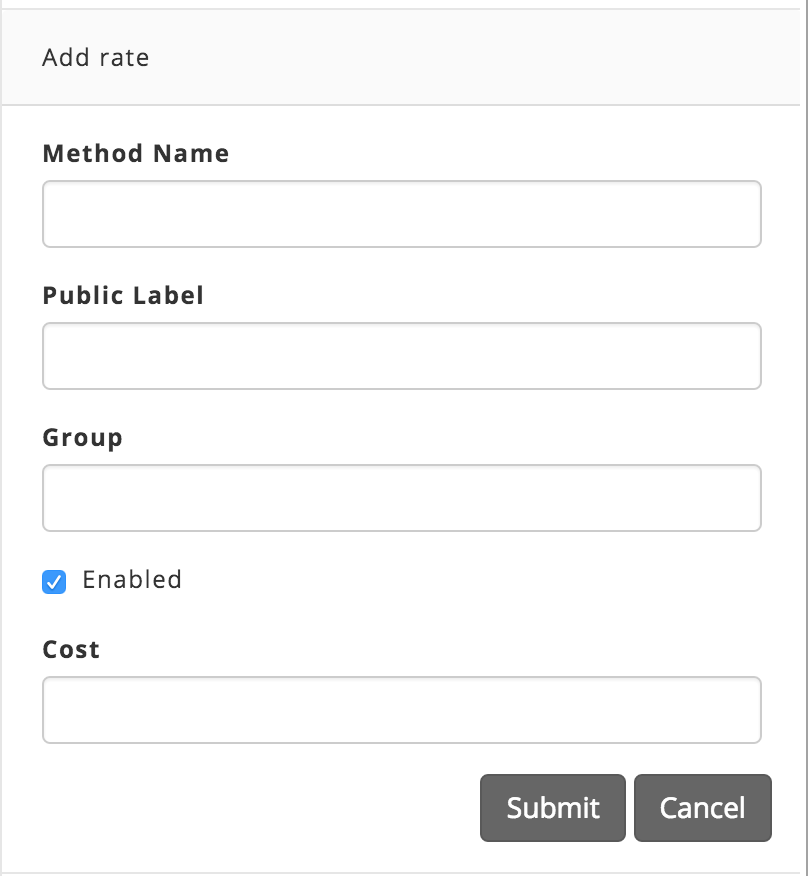
\includegraphics[width=0.6\textwidth]{figuras/dashboard/shipping/form_shipping_add.png}
	\caption{Formulario para la creación de \shippingEF.}
	\label{figure:dashboard:shipping:form_shipping_add}
\end{figure}



\begin{figure}[H]
	\centering
	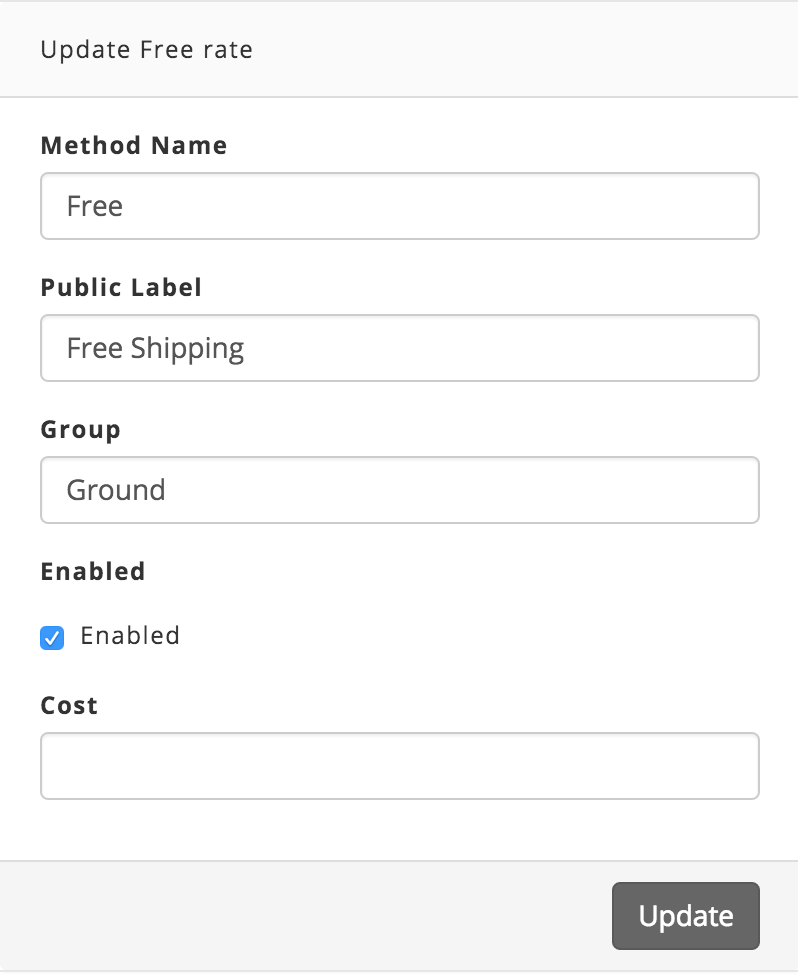
\includegraphics[width=0.6\textwidth]{figuras/dashboard/shipping/form_shipping_update.png}
	\caption{Formulario de actualización un \shippingEF.}
	\label{figure:dashboard:shipping:form_shipping_update}
\end{figure}


\subsubsection{Tarifas de \shippingEF y carros abadonados}

Aunque no es un tema que involucre a la finalidad de esta memoeria, es importante mencionar la importancia que tiene el factor \shippingEF dentro del abandono del carro de compra.
El desafio real que aparece cuando se desea abordar la estrategía de \shippingEF, es determinar la solución que lo mínimo posible los margenes, pero que aún asi siga siendo atractivo para el cliente.
Y esto es algo en lo que se va querer esta en lo correcto. Estudios demuestran que  tanto \shippingEF como manejar son la principal razón del abandano de carros de compra (\refFigura{figure:dashboard:shipping:key_factor_shopping_cart_abandonment})\cite{online_forrester_consulting_smarter_stratefie_free_shipping}.

\begin{figure}[H]
	\centering
	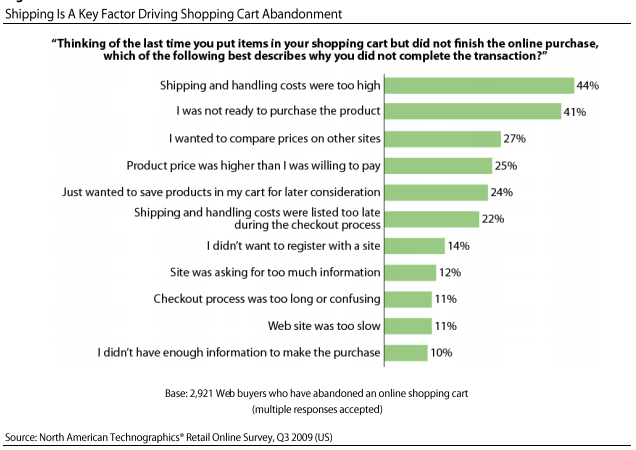
\includegraphics[width=1\textwidth]{figuras/dashboard/shipping/key_factor_shopping_cart_abandonment.png}
	\caption{\shippingEF es un factor clave hacia el abandono de carros de compra \cite{online_forrester_consulting_smarter_stratefie_free_shipping}.}
	\label{figure:dashboard:shipping:key_factor_shopping_cart_abandonment}
\end{figure}